\documentclass[
    english,
    % signatureplaces % prideda parašų vietas tituliniame puslapyje
]{VUMIFPSbakalaurinis}
\usepackage{float}
\usepackage{wrapfig2}
\usepackage{hyperref}
\usepackage{algorithmicx}
\usepackage{algorithm}
\usepackage{algpseudocode}
\usepackage{amsfonts}
\usepackage{amsmath}
\usepackage{bm}
\usepackage{caption}
\usepackage{color}
\usepackage{graphicx}
\usepackage{listings}
\usepackage{subcaption}
\usepackage{biblatex}
\usepackage{booktabs}
\usepackage{csquotes}

% Titulinio aprašas
\university{Vilnius University}
\faculty{Faculty of Mathematics and Informatics}
\department{Software Engineering Bachelor's Study Programme}
\papertype{Bachelor's Thesis}
\title{Vaizdų transformerių tinklų pritaikymas vaizdų panašumo vertinimui naudojant metrikų mokymąsi}
\titleineng{Vision Transformer Fine-Tuning for Image Similarity Using Metric Learning}
\author{Vytautas Mielkus}
\supervisor{lect. Boleslovas Dapkūnas}
\reviewer{prof. Olga Kurasova}
\date{Vilnius – \the\year}

\bibliography{bibliografija}

\begin{document}
\maketitle

% Turinys
\tableofcontents

% ============================================================================
% Santrauka (Lithuanian Abstract)
% ============================================================================
\sectionnonum{Santrauka}

Vaizdų panašumo aptikimas yra fundamentali kompiuterinės regos užduotis, taikoma turinio moderavime, autorių teisių apsaugoje ir dezinformacijos stebėjime. Šiame darbe tiriama, kaip skirtingos metrinės mokymosi nuostolių funkcijos veikia DINOv2 vizualinio transformerio tinklo tikslinimą vaizdų panašumo uždaviniui.

Eksperimentuose naudojamas DISC21 duomenų rinkinys – didelio masto vaizdų kopijų aptikimo etalonas. Tirtos penkios nuostolių funkcijos – kontrastyvinė, tripletų, ArcFace, židinio (Focal) ir CLIP/InfoNCE – pritaikytos abiejų DINOv2 modelio variantų: ViT-S/14 (21M parametrų) ir ViT-B/14 (86M parametrų) tikslinimui. Iš viso atlikti 12 eksperimentinių konfigūracijų, lyginant rezultatus pagal Precision@K, vidutinę vidutinę tikslumą (mAP) ir mikro vidutinę tikslumą (μAP) metrikas. Papildomai atlikta įterpimo erdvės analizė naudojant UMAP projekcijas ir kosinusinio panašumo skirstinių histogramas.

Eksperimentų rezultatai rodo, kad CLIP/InfoNCE nuostolių funkcija pasiekia geriausius rezultatus abiem modelio variantams: ViT-S P@1 = 60,49\%, ViT-B P@1 = 61,63\%. Tripletų nuostolių funkcija nepateikia mokymosi signalo nė vienam iš modelių, nes DINOv2 apdoroti įterpimai jau tenkina ribinę sąlygą. ViT-B modelis, nepaisant didesnio parametrų skaičiaus, ne visada lenkia ViT-S: kontrastyvinės nuostolių funkcijos atveju ViT-B pralenkia ViT-S net 4,91 procentiniais punktais P@1, o tripletų atveju skirtumas nereikšmingas.

\textbf{Raktiniai žodžiai:} vizualinis transformeris, metriniai mokymasis, vaizdų panašumas, DINOv2, kontrastyvinė nuostolių funkcija, ArcFace, CLIP, DISC21.

% ============================================================================
% Summary (English Abstract)
% ============================================================================
\sectionnonum{Summary}

\textbf{Vision Transformer Fine-Tuning for Image Similarity Using Metric Learning}

Image similarity detection is a fundamental computer vision task applied in content moderation, copyright enforcement, and misinformation tracking. This thesis investigates how different metric learning loss functions affect the fine-tuning of a DINOv2 Vision Transformer for image similarity tasks.

Experiments are conducted on the DISC21 dataset, a large-scale benchmark for image copy detection. Five loss functions---contrastive, triplet, ArcFace, Focal, and CLIP/InfoNCE---are evaluated across two DINOv2 backbone variants: ViT-S/14 (21M parameters) and ViT-B/14 (86M parameters), yielding 12 experimental configurations. Models are assessed using Precision@K, mean Average Precision (mAP), and micro Average Precision (μAP) metrics. Embedding space structure is further examined through UMAP projections and cosine similarity distribution histograms.

Results show that CLIP/InfoNCE achieves the best performance on both backbones: ViT-S P@1 = 60.49\%, ViT-B P@1 = 61.63\%. Triplet loss provides no learning signal for either backbone, as DINOv2's pre-trained embeddings already satisfy the margin constraint. The ViT-B backbone does not uniformly outperform ViT-S: contrastive loss benefits substantially from the larger backbone (+4.91 percentage points in P@1), while the advantage is negligible for triplet loss.

\textbf{Keywords:} vision transformer, metric learning, image similarity, DINOv2, contrastive loss, ArcFace, CLIP, DISC21.

% ============================================================================
% Abbreviations
% ============================================================================
\sectionnonum{Abbreviations}

\begin{description}
    \item[CLIP] Contrastive Language-Image Pre-training
    \item[CNN] Convolutional Neural Network
    \item[DISC21] Image Similarity Challenge 2021 dataset
    \item[DINOv2] Data-efficient Image Transformers v2 (self-supervised learning framework by Meta AI)
    \item[InfoNCE] Noise-Contrastive Estimation loss used in contrastive predictive coding
    \item[mAP] Mean Average Precision
    \item[μAP] Micro Average Precision (official DISC21 metric)
    \item[MLP] Multi-Layer Perceptron
    \item[SSL] Self-Supervised Learning
    \item[t-SNE] t-distributed Stochastic Neighbor Embedding
    \item[UMAP] Uniform Manifold Approximation and Projection
    \item[ViT] Vision Transformer
    \item[ViT-S] Vision Transformer Small variant (21M parameters)
    \item[ViT-B] Vision Transformer Base variant (86M parameters)
\end{description}

% ============================================================================
% Introduction
% ============================================================================
\sectionnonum{Introduction}

Image similarity detection is a fundamental computer vision task with significant practical applications in content moderation, copyright enforcement, and misinformation tracking on social media platforms \cite{Dou21}. The task involves determining whether a query image is a modified copy of any image in a reference database, where modifications may include cropping, filtering, rotation, text overlays, or other transformations.

Figure~\ref{fig:disc21_examples} illustrates concrete examples from the DISC21 dataset \cite{Dou21}. Each query image on the left is a modified version of the corresponding reference image on the right. The modifications include cropping, color adjustments, and composition changes. Despite these transformations, an effective similarity detection system should be able to match the query to its source reference.

\begin{figure}[H]
    \centering
    \begin{tabular}{cc}
        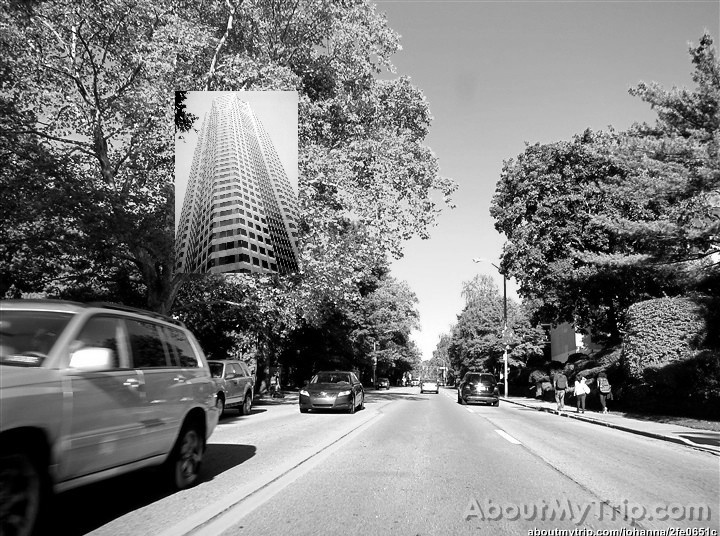
\includegraphics[height=0.2\textheight]{img/examples/Q00061.jpg} &
        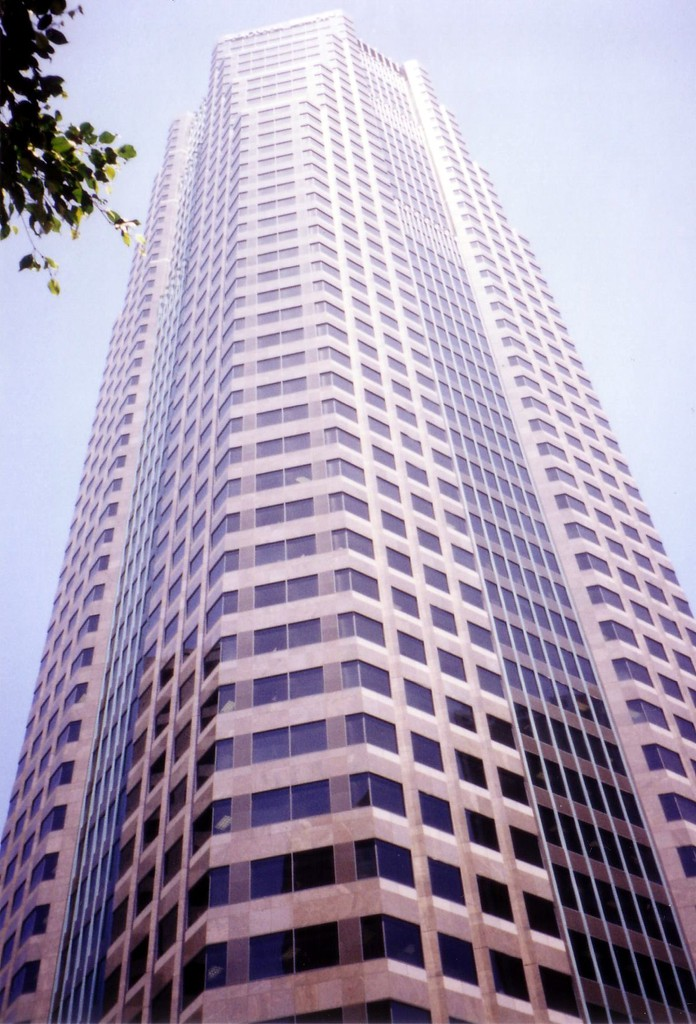
\includegraphics[height=0.2\textheight]{img/examples/R020965.jpg} \\
        (a) Query image Q00061 & (b) Reference image R020965 \\[1em]
        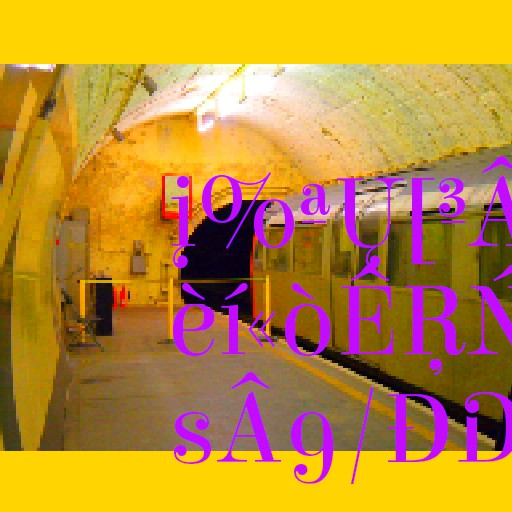
\includegraphics[height=0.2\textheight]{img/examples/Q00338.jpg} &
        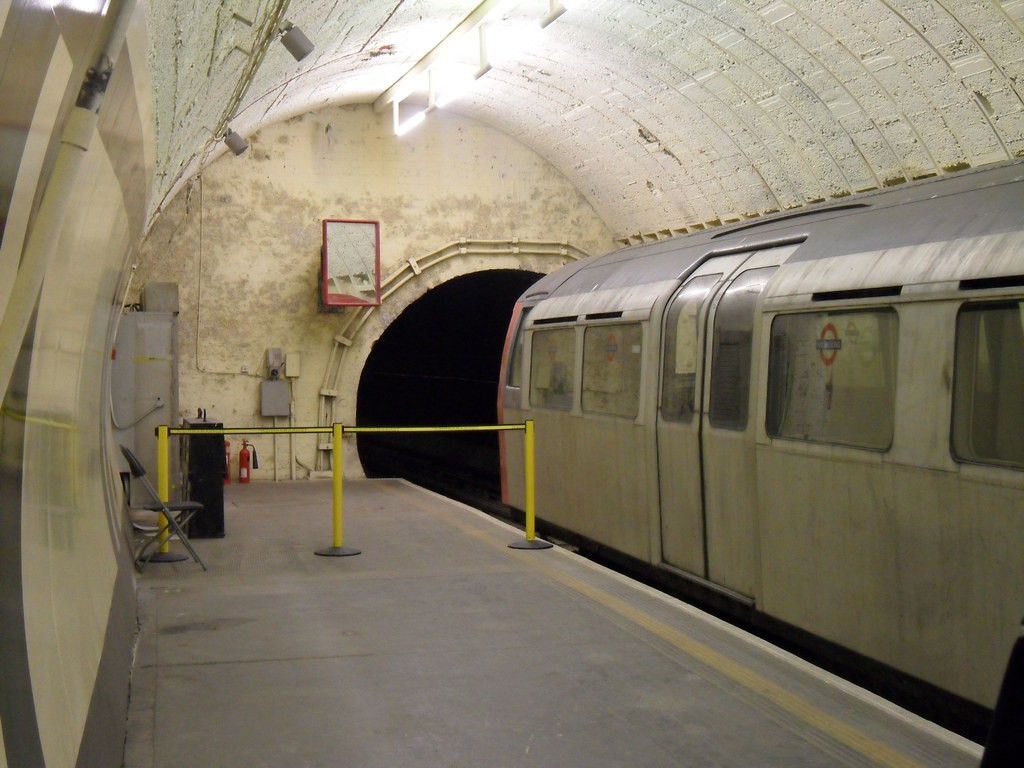
\includegraphics[height=0.2\textheight]{img/examples/R003142.jpg} \\
        (c) Query image Q00338 & (d) Reference image R003142 \\
    \end{tabular}
    \caption{Examples of query-reference pairs from the DISC21 dataset. Queries (left) are modified versions of references (right). The task is to correctly match each query to its source reference.}
    \label{fig:disc21_examples}
\end{figure}

Recent advances in self-supervised learning have produced powerful visual feature extractors that can be applied to similarity detection tasks. DINOv2 \cite{Oqu24}, developed by Meta AI, represents the state-of-the-art in learning robust visual features without supervision. Built on the Vision Transformer (ViT) architecture \cite{Dos21}, DINOv2 produces embeddings that capture semantic image content while remaining invariant to various transformations.

The choice of loss function during fine-tuning significantly impacts the quality of learned embeddings for similarity tasks. Metric learning approaches such as contrastive loss \cite{Che20}, triplet loss \cite{Sch15}, ArcFace loss \cite{Den22}, Focal loss \cite{Lin17}, and CLIP/InfoNCE loss \cite{Oor18} each offer different strategies for learning discriminative embeddings, originating from domains including face recognition, object detection, and multimodal learning. Understanding their comparative effectiveness across different backbone capacities is important for developing practical image similarity systems.

\textbf{The aim of this work} is to compare the effectiveness of different metric learning loss functions and Vision Transformer backbone sizes for fine-tuning a pre-trained DINOv2 model on the image similarity task.

\textbf{Objectives:}
\begin{enumerate}
    \item Establish baselines by evaluating two pre-trained DINOv2 variants---ViT-S/14 and ViT-B/14---without fine-tuning.
    \item Implement and train models using five loss functions: contrastive loss, triplet loss, ArcFace loss, Focal loss, and CLIP/InfoNCE loss, for both backbone variants.
    \item Evaluate all models using standard retrieval metrics: Precision@K, mean Average Precision (mAP), and micro Average Precision ($\mu$AP).
    \item Analyze the embedding space structure of the trained models using cosine similarity distributions and UMAP projections.
    \item Compare results across loss functions and backbone sizes to determine which combination is most effective for image similarity.
\end{enumerate}

% ============================================================================
% SECTION 1: SIMILARITY SEARCH
% ============================================================================
\section{Similarity Search}
\label{sec:similarity_search}

This section explains the key concepts needed to understand the image similarity methods used in this work. The section begins with the Transformer architecture, then explains how it was adapted for images (Vision Transformers), discusses self-supervised learning, and finally describes the loss functions used for training.

\subsection{Transformer Architecture}

The Transformer is a neural network architecture introduced by Vaswani et al. \cite{Vas17} in 2017. It was originally designed for text processing tasks like translation. The key idea is the \textbf{attention mechanism}, which allows the model to look at all parts of the input at once and decide which parts are most important for each output.

Before Transformers, most text models processed words one by one in order (like reading a sentence from left to right). This was slow and made it hard for the model to connect words that were far apart in a sentence. Transformers solve this by processing all words at the same time and using attention to find connections between any words, regardless of their position.

\subsubsection{Attention Mechanism}

The attention mechanism is the core idea behind Transformers. In simple terms, attention answers the question: \enquote{When processing this part of the input, which other parts should I pay attention to?}

Vaswani et al. \cite{Vas17} define the attention function using three components:
\begin{itemize}
    \item \textbf{Query (Q)}: What is being searched for
    \item \textbf{Key (K)}: What each element offers
    \item \textbf{Value (V)}: The actual content to retrieve
\end{itemize}

The formula for computing attention, as defined in the original paper \cite{Vas17}, is:

\begin{equation}
\text{Attention}(Q, K, V) = \text{softmax}\left(\frac{QK^T}{\sqrt{d_k}}\right)V
\label{eq:attention}
\end{equation}

The attention mechanism computes a similarity score between each query and all keys through the $QK^T$ operation, normalizes these scores to sum to 1 using the softmax function, and uses the resulting weights to create a weighted combination of values. The division by $\sqrt{d_k}$ (where $d_k$ is the dimension of the key vectors) serves as a scaling factor to prevent the dot product values from becoming too large, which stabilizes the gradient flow during training.

\textbf{Multi-head attention} runs several attention operations in parallel, each learning to focus on different types of relationships. For example, one \enquote{head} might learn to connect subjects with verbs, while another connects adjectives with nouns. The outputs are combined at the end.

\subsubsection{Transformer Encoder Structure}

The Transformer encoder is built by stacking multiple identical layers. Each layer has two main parts:
\begin{enumerate}
    \item \textbf{Attention layer}: Lets each position look at all other positions
    \item \textbf{Feed-forward layer}: Processes each position independently
\end{enumerate}

Between these parts, the model uses \enquote{residual connections} (adding the input back to the output) and \enquote{layer normalization} (keeping values in a reasonable range). Figure~\ref{fig:transformer} shows this structure.

\begin{figure}[H]
\centering
\fbox{\parbox{0.7\textwidth}{
\centering
\textbf{Transformer Encoder Block}\\[0.5em]
\begin{tabular}{c}
Input \\
$\downarrow$ \\
\fbox{Multi-Head Attention} \\
$\downarrow$ (add input back + normalize) \\
\fbox{Feed-Forward Network} \\
$\downarrow$ (add input back + normalize) \\
Output \\[0.3em]
\textit{(this block is repeated $N$ times)}
\end{tabular}
}}
\caption{Structure of a Transformer encoder block, as described in \cite{Vas17}.}
\label{fig:transformer}
\end{figure}

\subsection{Vision Transformers}

The ViT was introduced by Dosovitskiy et al. \cite{Dos21} in 2020. The main idea is to adapt the Transformer architecture, originally designed for sequential text data, to process images. However, images are not sequences of words, so the architecture must be adapted accordingly.

\subsubsection{Treating Images as Sequences}

The solution is to split the image into small square pieces called \textbf{patches}. For example, a 224$\times$224 pixel image can be divided into 196 patches of 16$\times$16 pixels each. Each patch is then converted into a vector (a list of numbers), similar to how words are converted to vectors in text models.

The process works as follows:
\begin{enumerate}
    \item Split the image into $N$ non-overlapping patches (e.g., 14$\times$14 = 196 patches)
    \item Flatten each patch into a 1D vector
    \item Project each vector to a fixed size using a linear layer
    \item Add position information so the model knows where each patch came from
    \item Process through the Transformer encoder
\end{enumerate}

A special \enquote{classification token} [CLS] is added at the beginning. After processing, this token's output is used as the image representation. Figure~\ref{fig:vit} illustrates this process.

\begin{figure}[H]
\centering
\fbox{\parbox{0.8\textwidth}{
\centering
\textbf{ViT Process}\\[0.5em]
\begin{tabular}{c}
Input Image (e.g., 224$\times$224 pixels) \\
$\downarrow$ \\
Split into patches (e.g., 196 patches of 16$\times$16) \\
$\downarrow$ \\
Convert each patch to a vector \\
$\downarrow$ \\
Add [CLS] token + position information \\
$\downarrow$ \\
Process through Transformer layers \\
$\downarrow$ \\
Use [CLS] output as image representation
\end{tabular}
}}
\caption{How Vision Transformer processes an image, based on \cite{Dos21}.}
\label{fig:vit}
\end{figure}

\subsubsection{ViT Model Sizes}

ViT comes in different sizes, from small to huge. Larger models can learn more complex patterns but require more computing power. Table~\ref{tab:vit_variants} shows the standard configurations. The naming convention ViT-X/Y means variant X with patch size Y (e.g., ViT-S/14 is the Small model with 14$\times$14 patches).

\begin{table}[H]
\centering
\caption{Vision Transformer model sizes, as defined in \cite{Dos21}}
\label{tab:vit_variants}
\begin{tabular}{lcccc}
\toprule
\textbf{Model} & \textbf{Layers} & \textbf{Hidden Size} & \textbf{Heads} & \textbf{Parameters} \\
\midrule
ViT-S (Small) & 12 & 384 & 6 & 22M \\
ViT-B (Base) & 12 & 768 & 12 & 86M \\
ViT-L (Large) & 24 & 1024 & 16 & 307M \\
ViT-H (Huge) & 32 & 1280 & 16 & 632M \\
\bottomrule
\end{tabular}
\end{table}

In this work, both the ViT-S (Small) and ViT-B (Base) variants are evaluated to examine the effect of backbone capacity on image similarity performance.

\subsection{Self-Supervised Learning and DINOv2}

\textbf{Self-supervised learning} is a way to train neural networks without manually labeled data. Instead of telling the model \enquote{this image is a cat}, the model learns by solving tasks it creates for itself. For example, it might learn to match different views of the same image, or to predict missing parts of an image.

This is important because labeling millions of images is expensive and time-consuming. Self-supervised learning allows models to learn from huge amounts of unlabeled images from the internet.

\subsubsection{How DINO Works}

DINO (Self-\textbf{DI}stillation with \textbf{NO} labels) \cite{Car21} uses a clever training approach with two networks:

\begin{itemize}
    \item \textbf{Student network}: The model being trained
    \item \textbf{Teacher network}: A slowly-updated copy of the student
\end{itemize}

During training, both networks see the same image but with different random changes applied (cropping, color changes, etc.). The student tries to produce the same output as the teacher. Since the teacher changes slowly, it provides stable targets for the student to learn from.

This approach demonstrates strong performance: the model learns to recognize objects and scenes through self-supervised learning without explicit labels. The resulting image representations capture semantic meaning and visual features that are useful for downstream tasks.

\subsubsection{DINOv2}

DINOv2 \cite{Oqu24} is an improved version released by Meta AI in 2023. The main improvements are:

\begin{itemize}
    \item \textbf{More training data}: 142 million carefully selected images
    \item \textbf{Better training}: Combines multiple learning objectives
    \item \textbf{Multiple sizes}: From small (22M parameters) to giant (1.1B parameters)
\end{itemize}

The key advantage of DINOv2 for our task is that it produces image embeddings that are:
\begin{itemize}
    \item \textbf{Meaningful}: Similar images get similar embeddings
    \item \textbf{Robust}: Embeddings stay similar even when images are cropped, rotated, or color-adjusted
    \item \textbf{General}: Works well for many different tasks without task-specific training
\end{itemize}

These properties make DINOv2 well-suited for image similarity detection.

\subsection{Metric Learning and Loss Functions}

\textbf{Metric learning} is about teaching a neural network to measure similarity between images. The goal is to convert images into vectors (called embeddings) such that:
\begin{itemize}
    \item Similar images have embeddings that are \textbf{close together}
    \item Different images have embeddings that are \textbf{far apart}
\end{itemize}

This is illustrated in Figure~\ref{fig:metric_learning}. The key question is: how is a model trained to achieve this? The answer is through \textbf{loss functions} that define what \enquote{good} embeddings look like.

\begin{figure}[H]
\centering
\fbox{\parbox{0.8\textwidth}{
\centering
\textbf{Goal of Metric Learning}\\[0.5em]
\begin{tabular}{ccc}
\textbf{Before Training} & $\longrightarrow$ & \textbf{After Training} \\[0.5em]
Random embeddings & & Grouped by similarity \\
(images scattered randomly) & & (similar images close together)
\end{tabular}
}}
\caption{Metric learning teaches the model to place similar images close together in the embedding space.}
\label{fig:metric_learning}
\end{figure}

Three different loss functions were tested, each with a different approach to this problem. The formulas come from the original papers that introduced these methods.

\subsubsection{Contrastive Loss}

Contrastive loss was originally introduced by Hadsell et al. \cite{Had06} for learning invariant mappings through dimensionality reduction. The approach was later popularized in modern self-supervised learning frameworks such as SimCLR \cite{Che20}. Contrastive loss works with \textbf{pairs} of images. For each pair, it is known whether they should be similar (positive pair) or different (negative pair).

The formula \cite{Che20} is:
\begin{equation}
\mathcal{L}_{\text{contrastive}} = y \cdot d^2 + (1-y) \cdot \max(0, m - d)^2
\label{eq:contrastive}
\end{equation}

In plain terms:
\begin{itemize}
    \item $y = 1$ means \enquote{these images should be similar} $\rightarrow$ minimize the distance $d$
    \item $y = 0$ means \enquote{these images should be different} $\rightarrow$ push them apart until distance is at least $m$
\end{itemize}

The parameter $m$ (margin) defines how far apart negative pairs should be. Once they're far enough, the model stops pushing them further.

\subsubsection{Triplet Loss}

The concept of using triplets for metric learning has earlier roots in large margin nearest neighbor classification \cite{Wei06}. Triplet loss was popularized by Schroff et al. \cite{Sch15} in the FaceNet framework for face recognition. Triplet loss works with \textbf{three} images at a time:
\begin{itemize}
    \item \textbf{Anchor}: The reference image
    \item \textbf{Positive}: An image that should be similar to anchor
    \item \textbf{Negative}: An image that should be different from anchor
\end{itemize}

The formula \cite{Sch15} is:
\begin{equation}
\mathcal{L}_{\text{triplet}} = \max(0, d_{ap} - d_{an} + m)
\label{eq:triplet}
\end{equation}

The idea is simple: the anchor should be closer to the positive than to the negative, by at least a margin $m$. Figure~\ref{fig:triplet} illustrates this.

\begin{figure}[H]
\centering
\fbox{\parbox{0.7\textwidth}{
\centering
\textbf{Triplet Loss Requirement}\\[0.5em]
\begin{tabular}{c}
distance(Anchor, Positive) + margin $<$ distance(Anchor, Negative) \\[0.5em]
In other words: the similar image should be \\
closer than the different image, with some room to spare.
\end{tabular}
}}
\caption{Triplet loss requires the positive to be closer to the anchor than the negative by at least margin $m$.}
\label{fig:triplet}
\end{figure}

\textbf{Triplet mining} is important: if random triplets are selected, most will already satisfy the constraint (loss = 0) and the model learns nothing. \enquote{Hard} triplet mining finds difficult cases where the negative is closer than expected.

\subsubsection{ArcFace Loss}

ArcFace \cite{Den22} takes a different approach. Instead of comparing pairs or triplets, it treats each image as a separate class and trains a classifier. The clever part is adding an \textbf{angular margin} that forces the model to create well-separated clusters.

The formula from \cite{Den22} is complex:
\begin{equation}
\mathcal{L}_{\text{arcface}} = -\log \frac{e^{s \cdot \cos(\theta_{y} + m)}}{e^{s \cdot \cos(\theta_{y} + m)} + \sum_{j \neq y} e^{s \cdot \cos(\theta_j)}}
\label{eq:arcface}
\end{equation}

The key idea in simpler terms: the model learns to place each image's embedding close to its \enquote{class center} (a learned vector), and the margin $m$ ensures there's clear separation between different classes. The parameters $s$ (scale) and $m$ (margin) control how strict this separation should be.

Figure~\ref{fig:arcface} shows the difference from standard classification.

\begin{figure}[H]
\centering
\fbox{\parbox{0.75\textwidth}{
\centering
\textbf{ArcFace vs Standard Classification}\\[0.5em]
\begin{tabular}{cc}
\textbf{Standard} & \textbf{ArcFace} \\[0.3em]
Classes can be close together & Margin forces separation \\
May overlap at boundaries & Clear gaps between classes
\end{tabular}
}}
\caption{ArcFace adds a margin that forces clearer separation between image classes.}
\label{fig:arcface}
\end{figure}

\subsubsection{Focal Loss}

Focal loss was introduced by Lin et al. \cite{Lin17} as part of the RetinaNet object detector to address the class imbalance problem in dense object detection. The key insight is that standard cross-entropy loss assigns equal weight to all training samples, causing the loss to be dominated by easy, correctly classified examples that contribute little useful learning signal.

Focal loss addresses this by adding a modulating factor $(1 - p_t)^\gamma$ to the standard cross-entropy:

\begin{equation}
\mathcal{L}_{\text{focal}} = -\alpha_t (1 - p_t)^\gamma \log(p_t)
\label{eq:focal}
\end{equation}

where $p_t$ is the model's estimated probability for the true class, $\gamma \geq 0$ is the focusing parameter, and $\alpha_t$ is a class-weighting factor. When $\gamma = 0$, focal loss reduces to standard cross-entropy. As $\gamma$ increases, the relative weight of easy examples decreases, focusing training on hard, misclassified examples.

While focal loss originates from object detection, it is applicable to image similarity by treating each image as its own class (similar to ArcFace). The focusing mechanism encourages the model to concentrate on images that are difficult to classify, potentially learning more discriminative embeddings for hard cases.

\subsubsection{CLIP/InfoNCE Loss}

The InfoNCE loss was introduced by van den Oord et al. \cite{Oor18} as part of the Contrastive Predictive Coding framework and was later popularized at scale in the CLIP model by Radford et al. \cite{Rad21}. Unlike contrastive and triplet losses that operate on pairs or triplets, CLIP/InfoNCE is a batch-level loss that uses all samples in a batch as mutual negatives.

Given a batch of $N$ image pairs $(x_i, x_i^+)$ where $x_i^+$ is a positive view of $x_i$, the embeddings $z_i = f(x_i)$ and $z_i^+ = f(x_i^+)$ are computed. The loss for a single sample is:

\begin{equation}
\mathcal{L}_{\text{InfoNCE}}(i) = -\log \frac{\exp(\text{sim}(z_i, z_i^+) / \tau)}{\sum_{j=1}^{N} \exp(\text{sim}(z_i, z_j^+) / \tau)}
\label{eq:infonce}
\end{equation}

where $\text{sim}(\cdot, \cdot)$ is cosine similarity and $\tau > 0$ is a learnable or fixed temperature parameter. The final loss averages over all $N$ samples. The denominator sums over all $N$ samples in the batch, meaning each batch of size $N$ provides $N-1$ implicit negatives per sample.

The key advantage of InfoNCE over contrastive and triplet loss is the efficient use of batch structure: a batch of 256 samples provides 255 negatives per anchor, compared to just one for contrastive loss. The temperature $\tau$ controls the sharpness of the distribution; lower values make the loss more sensitive to fine-grained differences.

\subsubsection{Summary of Loss Functions}

Table~\ref{tab:loss_comparison} summarizes all five loss functions evaluated in this work.

\begin{table}[H]
\centering
\caption{Comparison of metric learning loss functions}
\label{tab:loss_comparison}
\begin{tabular}{lccccc}
\toprule
\textbf{Property} & \textbf{Contrastive} & \textbf{Triplet} & \textbf{ArcFace} & \textbf{Focal} & \textbf{CLIP/InfoNCE} \\
\midrule
Input type & Pairs & Triplets & Single & Single & Pairs \\
Mining needed & No & Yes & No & No & No \\
Formulation & Distance & Distance & Angular & Classification & Batch contrastive \\
Negatives per sample & 1 & 1 & $N_c - 1$ & $N_c - 1$ & $N - 1$ \\
Origin domain & Self-sup. & Face recog. & Face recog. & Object det. & Multimodal \\
\bottomrule
\end{tabular}
\end{table}

\subsection{Evaluation Metrics}

To measure how well the models perform at finding similar images, several standard metrics from information retrieval are used.

\subsubsection{Precision at K}

\textbf{Precision@K (P@K)} answers a simple question: \enquote{Is the correct match among the top K results?}

\begin{itemize}
    \item \textbf{P@1}: Is the \#1 result correct? (most strict)
    \item \textbf{P@5}: Is the correct match in the top 5?
    \item \textbf{P@10}: Is the correct match in the top 10?
\end{itemize}

The percentage of queries where this is true is calculated. For example, P@1 = 60\% means the correct match was ranked first for 60\% of queries.

The formula for Precision@K is:
\begin{equation}
\text{P@K} = \frac{1}{|\mathcal{Q}|} \sum_{q \in \mathcal{Q}} I[\text{rank}(q) \leq K]
\label{eq:patk}
\end{equation}
where $\mathcal{Q}$ is the set of queries, $\text{rank}(q)$ is the rank of the correct match for query $q$, and $I[\text{rank}(q) \leq K]$ equals 1 if the rank is at most $K$ and 0 otherwise.

\subsubsection{Mean Average Precision}

\textbf{Mean Average Precision (mAP)} measures not just whether the correct match is found, but how high it is ranked. A system that consistently ranks correct matches near the top will have a higher mAP than one that finds them but ranks them lower.

The formula for mAP is:
\begin{equation}
\text{mAP} = \frac{1}{|\mathcal{Q}|} \sum_{q \in \mathcal{Q}} \text{AP}(q)
\label{eq:map}
\end{equation}
where $\text{AP}(q)$ is the Average Precision for query $q$, calculated as:
\begin{equation}
\text{AP}(q) = \sum_{k=1}^{n} \text{Precision@k} \cdot \Delta\text{Recall@k}
\label{eq:ap}
\end{equation}
where $n$ is the total number of retrieved items, and $\Delta\text{Recall@k}$ is the change in recall at position $k$.

\subsubsection{Micro Average Precision}

\textbf{Micro Average Precision ($\mu$AP)} is the official metric used in the DISC21 challenge \cite{Dou21}. As explained in the DISC21 paper, this metric treats each query-reference pair equally, which is important for real-world scenarios where some queries might have multiple correct matches.

The formula for $\mu$AP \cite{Dou21} is:
\begin{equation}
\mu\text{AP} = \frac{1}{|\mathcal{P}|} \sum_{(q,r) \in \mathcal{P}} \text{AP}(q,r)
\label{eq:muap}
\end{equation}
where $\mathcal{P}$ is the set of positive query-reference pairs, and $\text{AP}(q,r)$ is the Average Precision for query $q$ with respect to reference $r$.

The DISC21 authors chose $\mu$AP because copy detection operates in a \enquote{needle in haystack} setting---most query images do not have matches, and when matches exist, finding them with high confidence matters more than finding all possible matches.

\subsection{Embedding Space Visualization}

While quantitative metrics measure retrieval performance, visualizing the learned embedding space provides additional qualitative insight into how loss functions shape the geometry of the feature space. Two complementary approaches are used in this work.

\subsubsection{Dimensionality Reduction}

\textbf{t-distributed Stochastic Neighbor Embedding (t-SNE)} \cite{van08} is a non-linear dimensionality reduction technique that maps high-dimensional embeddings to 2D while preserving local neighborhood structure. t-SNE converts pairwise distances into conditional probabilities and minimizes the Kullback-Leibler divergence between the high-dimensional and low-dimensional probability distributions. While t-SNE effectively reveals cluster structure, it does not preserve global distances between clusters.

\textbf{Uniform Manifold Approximation and Projection (UMAP)} \cite{McI18} is an alternative dimensionality reduction algorithm based on manifold learning theory. Compared to t-SNE, UMAP is faster to compute and better preserves global structure while still maintaining local neighborhood relationships. For large embedding sets, UMAP is preferred due to its computational efficiency.

Both methods are applied purely for qualitative analysis---the resulting 2D projections illustrate how well different loss functions separate matching from non-matching images in the learned embedding space, but the 2D coordinates themselves are not used for retrieval.

\subsubsection{Cosine Similarity Distributions}

A more direct and quantitative view of embedding space geometry is provided by plotting the distributions of cosine similarity scores for matching and non-matching image pairs. For each trained model, two distributions are computed from the development set:
\begin{itemize}
    \item \textbf{Matching pairs}: cosine similarity between a query and its correct reference image.
    \item \textbf{Non-matching pairs}: cosine similarity between a query and a randomly sampled, non-matching reference image.
\end{itemize}

The separation between these two distributions, defined as $\text{sep} = \bar{s}_{\text{match}} - \bar{s}_{\text{non-match}}$, provides a scalar summary of how well the model distinguishes true matches from distractors in embedding space. A larger separation indicates a more discriminative embedding.

% ============================================================================
% SECTION 2: METHODOLOGY
% ============================================================================
\section{Methodology}

This section describes the dataset, model architecture, and experimental setup used in this work.

\subsection{DISC21 Dataset}

The DISC21 dataset \cite{Dou21} was created by Meta AI for the Image Similarity Challenge at NeurIPS 2021. It is designed to evaluate large-scale image copy detection systems in realistic scenarios.

The dataset is organized into two main types of images:
\begin{itemize}
    \item \textbf{Query images}: Modified or transformed versions of original images. These represent the images that need to be matched to their source.
    \item \textbf{Reference images}: Original, unmodified images that serve as the database to search against. Each query image should be matched to its corresponding reference image.
\end{itemize}

The dataset contains over 2 million images with various transformations applied to query images, including:
\begin{itemize}
    \item Geometric transformations: crops, rotations, flips, scaling
    \item Photometric changes: color filters, brightness/contrast adjustments
    \item Overlays: text, logos, borders, watermarks
    \item Complex edits: collages, memes, screenshots
    \item Adversarial perturbations: designed to fool detection systems
\end{itemize}

For this work, a subset of approximately 50,000 images per category was used due to computational constraints (see Table~\ref{tab:dataset}).

\begin{table}[H]
\centering
\caption{DISC21 dataset subset used in experiments}
\label{tab:dataset}
\begin{tabular}{lrl}
\toprule
\textbf{Split} & \textbf{Images} & \textbf{Purpose} \\
\midrule
Training set & 50,000 & Fine-tuning with loss functions \\
Reference set & 50,000 & Database to search against \\
Development queries & 50,000 & Model validation and tuning \\
Test queries & 50,000 & Final evaluation \\
\bottomrule
\end{tabular}
\end{table}

Ground truth files provide 10,000 query-to-reference mappings for both development and test sets, indicating which queries match which references.

\subsection{Model Architecture}

The model architecture consists of a pre-trained DINOv2 backbone followed by a trainable projection head (see Figure~\ref{fig:architecture}). Two backbone variants are evaluated to study the effect of model capacity on similarity performance.

\begin{figure}[H]
\centering
\fbox{\parbox{0.85\textwidth}{
\centering
\textbf{Model Architecture}\\[0.5em]
\begin{tabular}{cc}
\textbf{ViT-S/14 variant} & \textbf{ViT-B/14 variant} \\[0.3em]
Input Image ($224 \times 224 \times 3$) & Input Image ($224 \times 224 \times 3$) \\
$\downarrow$ & $\downarrow$ \\
DINOv2 ViT-S/14 (21M params, frozen) & DINOv2 ViT-B/14 (86M params, frozen) \\
384-dim features & 768-dim features \\
$\downarrow$ & $\downarrow$ \\
Projection Head: $384 \rightarrow 128$ & Projection Head: $768 \rightarrow 128$ \\
$\downarrow$ & $\downarrow$ \\
\multicolumn{2}{c}{L2 Normalization} \\
\multicolumn{2}{c}{$\downarrow$} \\
\multicolumn{2}{c}{128-dimensional unit-length embedding}
\end{tabular}
}}
\caption{Model architecture for ViT-S/14 and ViT-B/14 variants. Both share the same projection head and L2 normalization design; only the backbone and input feature dimension differ.}
\label{fig:architecture}
\end{figure}

Table~\ref{tab:backbone_comparison} summarizes the key properties of both backbone variants.

\begin{table}[H]
\centering
\caption{DINOv2 backbone variants used in this work}
\label{tab:backbone_comparison}
\begin{tabular}{lcccc}
\toprule
\textbf{Backbone} & \textbf{Parameters} & \textbf{Feature dim.} & \textbf{Patch size} & \textbf{Layers} \\
\midrule
DINOv2 ViT-S/14 & 21M & 384 & $14 \times 14$ & 12 \\
DINOv2 ViT-B/14 & 86M & 768 & $14 \times 14$ & 12 \\
\bottomrule
\end{tabular}
\end{table}

During training, both DINOv2 backbones are kept frozen. Only the projection head is trained. This approach prevents catastrophic forgetting: the backbones were pre-trained on 142 million carefully curated images and have already learned robust visual features. Fine-tuning the entire model would risk overwriting these representations. By freezing the backbone, the pre-trained knowledge is preserved while the small projection head is optimized for the similarity detection task.

The projection head reduces the backbone's feature dimension to 128. This uniform output size allows direct comparison across both backbone variants and speeds up the similarity computation at evaluation time. L2 normalization ensures all embeddings lie on the unit hypersphere, which is required for cosine similarity computation.

\subsection{Data Augmentation}

Data augmentation plays a crucial role in metric learning by creating positive pairs from single images. During training, the following augmentations were applied:

\begin{itemize}
    \item \textbf{Random Resized Crop}: Images were randomly cropped to 80-100\% of the original area and resized to 224$\times$224 pixels.
    \item \textbf{Horizontal Flip}: Applied with 50\% probability.
    \item \textbf{Color Jitter}: Random adjustments to brightness ($\pm$20\%), contrast ($\pm$20\%), saturation ($\pm$20\%), and hue ($\pm$10\%).
\end{itemize}

All images were normalized using ImageNet mean and standard deviation values. This normalization step is a preprocessing operation rather than data augmentation, as it standardizes the input distribution without introducing variability.

For evaluation, only deterministic center cropping and normalization were applied to ensure reproducible results.

\subsection{Experimental Setup}

All experiments were conducted on the VU MIF HPC cluster using NVIDIA Tesla V100 GPUs with 32GB memory. The PyTorch Metric Learning library \cite{Mus20} was used for implementing the loss functions and mining strategies. The complete implementation code is available in the GitHub repository\footnote{\texttt{https://github.com/whz1gud/Kursinis}}. Training parameters are summarized in Table~\ref{tab:training}.

\begin{table}[H]
\centering
\caption{Training hyperparameters}
\label{tab:training}
\begin{tabular}{ll}
\toprule
\textbf{Parameter} & \textbf{Value} \\
\midrule
Optimizer & AdamW (weight decay = 0.01) \\
Learning rate & $4 \times 10^{-4}$ \\
Learning rate schedule & Cosine annealing with warm restarts \\
Epochs & 20 \\
Embedding dimension & 128 \\
Backbone & Frozen (ViT-S/14 or ViT-B/14) \\
\midrule
\multicolumn{2}{l}{\textit{Loss-specific parameters}} \\
Margin (contrastive / triplet) & 0.5 \\
ArcFace scale $s$ & 64 \\
ArcFace margin $m$ & 0.5 \\
Focal loss $\gamma$ & 2 \\
Focal loss $\alpha$ & 0.25 \\
InfoNCE temperature $\tau$ & 0.07 \\
\midrule
\multicolumn{2}{l}{\textit{Batch sizes (HPC, V100 32GB)}} \\
Contrastive / CLIP (ViT-S) & 256 \\
Triplet / ArcFace / Focal (ViT-S) & 1024 \\
Contrastive / CLIP (ViT-B) & 256 \\
Triplet / ArcFace / Focal (ViT-B) & 512 \\
\bottomrule
\end{tabular}
\end{table}

For contrastive and CLIP/InfoNCE losses, positive pairs were created by applying data augmentation to the same image twice, producing two different views of the same content. Negative pairs were sampled from different images within the same batch. For contrastive loss, one explicit negative is used per anchor; for CLIP/InfoNCE, all other samples in the batch serve as implicit negatives. For triplet loss, hard negative mining was employed to select the most challenging triplets.

For ArcFace and Focal losses, each training image was treated as its own class, transforming the similarity learning problem into a classification problem with 50,000 classes. ArcFace uses angular margin to encourage separation; Focal loss applies a modulating factor $(1-p_t)^\gamma$ to focus learning on hard examples.

\subsection{Evaluation Protocol}

The evaluation pipeline consists of the following steps:

\begin{enumerate}
    \item \textbf{Feature Extraction}: Extract 128-dimensional embeddings for all query and reference images using the trained model.
    \item \textbf{Similarity Computation}: Compute cosine similarity between each query embedding and all reference embeddings.
    \item \textbf{Ranking}: For each query, rank all references by descending similarity score.
    \item \textbf{Metric Calculation}: Compare rankings against ground truth to compute P@K, mAP, and $\mu$AP.
\end{enumerate}

Evaluation was performed every 5 epochs on the development query set. The model checkpoint with the best mAP score was saved for final evaluation. Feature extraction for 100,000 images (50,000 queries + 50,000 references) took approximately 6 minutes on a V100 GPU.

\subsection{Embedding Visualization Methodology}

To complement the quantitative metrics, the embedding spaces of all 12 trained models are visualized using two methods described in Section~\ref{sec:similarity_search}.

For cosine similarity distributions, all 50,000 development query embeddings are extracted and matched against the 50,000 reference embeddings. For each query, the cosine similarity to its correct reference (matching pair) and to a randomly sampled non-matching reference (non-matching pair) is recorded. The resulting distributions are plotted as density-normalized histograms and summarized by their means and separation $\text{sep} = \bar{s}_{\text{match}} - \bar{s}_{\text{non-match}}$.

For the UMAP projection, a stratified subsample of 500 development query embeddings is drawn from each model. UMAP is applied with parameters $n\_\text{neighbors} = 15$ and $\text{min\_dist} = 0.1$ to project the 128-dimensional embeddings to 2D. Points are color-coded by whether they correspond to a query with a correctly retrieved match at rank 1 (correct) or not (incorrect). All visualization scripts run on CPU and require no GPU.

% ============================================================================
% SECTION 3: EXPERIMENTS AND RESULTS
% ============================================================================
\section{Experiments and Results}

This section presents experimental results comparing baseline DINOv2 models with models fine-tuned using five different loss functions on two backbone variants. Training dynamics are analyzed, final performance metrics are compared across all 12 configurations, and the implications of the findings are discussed.

\subsection{Baseline Evaluation}

Baselines were established by evaluating both pre-trained DINOv2 variants without any fine-tuning. Features were extracted using the frozen backbone followed by a randomly initialized projection head.

Both baselines achieve strong performance without task-specific training, demonstrating that DINOv2's pre-trained features are already well-suited for image similarity tasks:
\begin{itemize}
    \item \textbf{ViT-S/14 baseline}: P@1 = 56.71\%, mAP = 58.80\%, $\mu$AP = 41.44\%
    \item \textbf{ViT-B/14 baseline}: P@1 = 57.84\%, mAP = 60.93\%, $\mu$AP = 39.92\%
\end{itemize}

The ViT-B/14 baseline already outperforms ViT-S/14 on P@1 (+1.13 pp) and mAP (+2.13 pp), reflecting the larger backbone's greater representational capacity. Interestingly, ViT-S/14 baseline achieves slightly higher $\mu$AP (41.44\% vs.\ 39.92\%), suggesting the smaller model's geometry may align differently with the DISC21 evaluation criterion.

\subsection{Training Dynamics}

Figure~\ref{fig:training_curves_main} shows the training loss curves for the ViT-S experiments over 20 epochs. The curves reveal distinctly different learning behaviors across loss functions.

\begin{figure}[H]
    \centering
    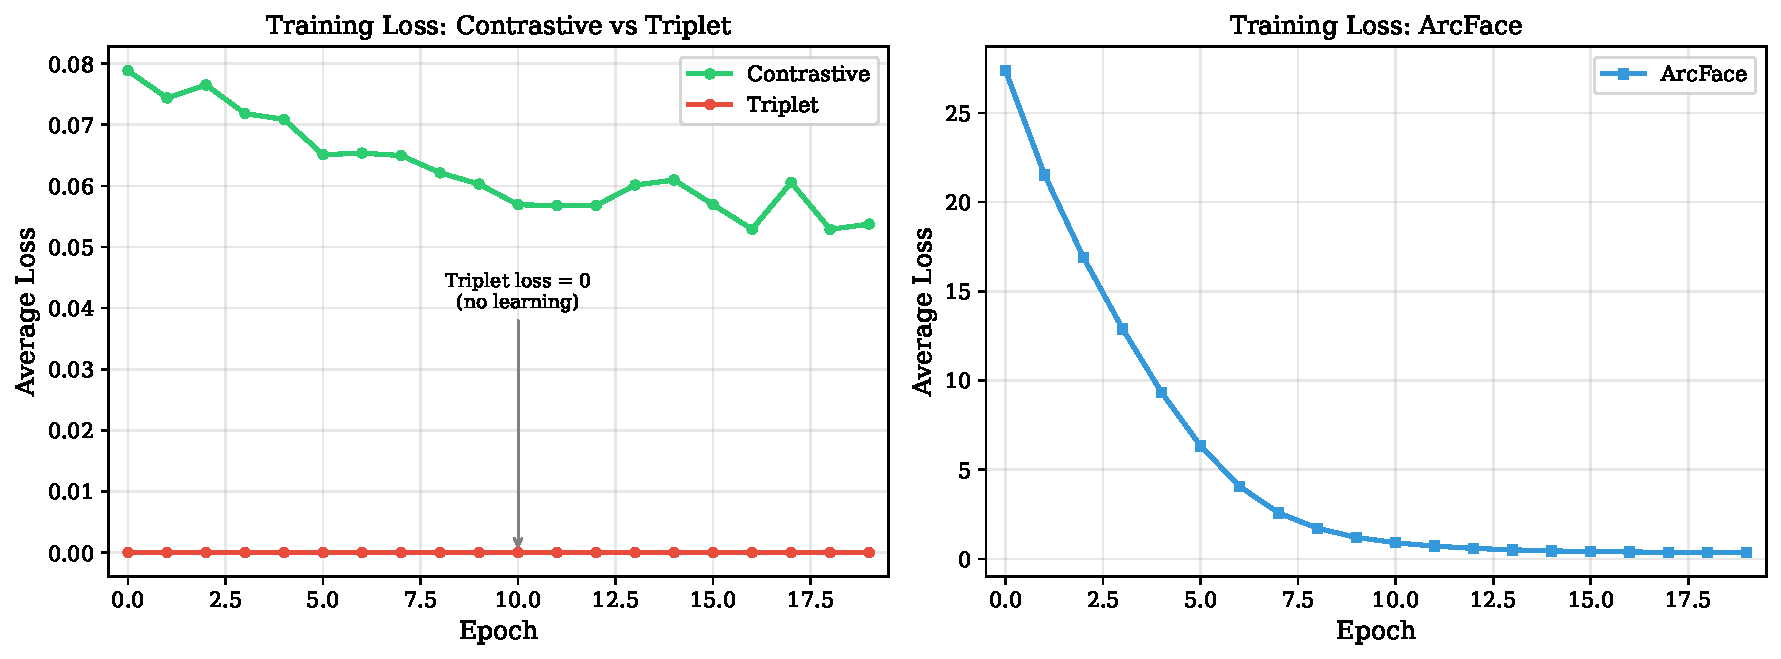
\includegraphics[width=\textwidth]{img/training_curves.pdf}
    \caption{Training loss curves for ViT-S experiments. Left: Contrastive and Triplet losses (same scale). Right: ArcFace loss (different scale due to higher initial values).}
    \label{fig:training_curves_main}
\end{figure}

Key observations:
\begin{itemize}
    \item \textbf{Contrastive loss} decreases gradually from 0.079 to 0.054, indicating stable convergence.
    \item \textbf{Triplet loss} remains at exactly 0.0 throughout training — a result analyzed in Section~\ref{sec:triplet_analysis}.
    \item \textbf{ArcFace loss} drops rapidly from 27.36 to approximately 0.35, providing a strong learning signal throughout.
    \item \textbf{Focal loss} (not shown) shows behavior similar to ArcFace, with rapid initial decrease from high cross-entropy values.
    \item \textbf{CLIP/InfoNCE loss} (not shown) decreases steadily, benefiting from the large number of in-batch negatives.
\end{itemize}

\subsection{Fine-tuning with Contrastive Loss}

Training with contrastive loss uses augmented views of the same image as positive pairs and other images in the batch as negatives. Results show mixed performance relative to baseline:
\begin{itemize}
    \item \textbf{ViT-S}: P@1 decreased by 1.32 pp (56.71\% $\rightarrow$ 55.39\%), but $\mu$AP \textbf{improved} by 6.46 pp (41.44\% $\rightarrow$ 47.90\%)
    \item \textbf{ViT-B}: P@1 \textbf{improved} by 2.46 pp (57.84\% $\rightarrow$ 60.30\%), $\mu$AP improved by 11.45 pp
\end{itemize}

The ViT-S result suggests that with a smaller backbone, contrastive training improves broad retrieval coverage ($\mu$AP) at the expense of precise top-1 accuracy. The ViT-B result is notably different: the larger backbone benefits substantially from contrastive fine-tuning, achieving the second-best P@1 among all ViT-B configurations.

\subsection{Fine-tuning with Triplet Loss}
\label{sec:triplet_analysis}

An unexpected result is observed with triplet loss training: the loss remains at exactly 0.0 throughout all 20 epochs for \textit{both} backbone variants. This indicates that the hard triplet mining strategy cannot find any triplets that violate the margin constraint.

\textbf{Why did this happen?} DINOv2's pre-trained embeddings are already highly discriminative. For all potential triplets in the training data, the positive (augmented view of the same image) is already much closer to the anchor than any negative, by more than the margin $m = 0.5$:
\begin{equation}
d(a, p) + m < d(a, n) \quad \text{(margin constraint already satisfied for all triplets)}
\end{equation}

Since $\mathcal{L}_{\text{triplet}} = \max(0, d(a,p) - d(a,n) + m) = 0$ for all triplets, no gradient is produced and no learning occurs. A follow-up experiment on ViT-S with $m = 1.0$ confirmed that the loss remained at 0.0, and metrics were essentially identical to the baseline.

As a result, triplet-trained models perform nearly identically to their respective baselines: ViT-S triplet achieves P@1 = 55.58\% and ViT-B triplet achieves P@1 = 58.41\%, with minimal change across all metrics. This finding highlights an important limitation of triplet loss when fine-tuning highly capable pre-trained models.

\subsection{Fine-tuning with ArcFace Loss}

ArcFace loss shows strong learning dynamics, with rapid initial decrease (ViT-S: from 27.36 to 0.35 over 20 epochs). The high initial loss is expected given 50,000 classification classes with random initial weights. Results show consistent improvement for both backbones:
\begin{itemize}
    \item \textbf{ViT-S}: P@1 = 58.41\% (+1.70 pp), mAP = 60.41\% (+1.61 pp), $\mu$AP = 48.82\% (+7.38 pp)
    \item \textbf{ViT-B}: P@1 = 59.17\% (+1.33 pp), mAP = 61.43\% (+0.50 pp), $\mu$AP = 43.27\% (+3.35 pp)
\end{itemize}

ArcFace provides a consistent learning signal because the angular margin formulation creates a well-defined objective even when the pre-trained embeddings are already discriminative. However, it is surpassed by CLIP/InfoNCE in all configurations.

\subsection{Fine-tuning with Focal Loss}

Focal loss treats each image as its own class (same as ArcFace) but modulates the cross-entropy by $(1-p_t)^2$, focusing the loss on hard-to-classify examples. Results show modest improvements over baseline:
\begin{itemize}
    \item \textbf{ViT-S}: P@1 = 56.52\% ($-$0.19 pp), mAP = 58.64\% ($-$0.16 pp), $\mu$AP = 43.93\% (+2.49 pp)
    \item \textbf{ViT-B}: P@1 = 58.79\% (+0.95 pp), mAP = 61.37\% (+0.44 pp), $\mu$AP = 45.86\% (+5.94 pp)
\end{itemize}

The focusing mechanism provides moderate gains in $\mu$AP but does not match ArcFace or CLIP/InfoNCE in P@1. For ViT-S, P@1 slightly decreases below baseline, suggesting the focusing parameter $\gamma = 2$ may push the model toward hard examples at the cost of common-case accuracy.

\subsection{Fine-tuning with CLIP/InfoNCE Loss}

CLIP/InfoNCE loss uses all $N-1$ other samples in a batch as implicit negatives, providing a richer learning signal per update step. Results consistently outperform all other loss functions:
\begin{itemize}
    \item \textbf{ViT-S}: P@1 = 60.49\% (+3.78 pp), mAP = 63.13\% (+4.33 pp), $\mu$AP = 48.80\% (+7.36 pp)
    \item \textbf{ViT-B}: P@1 = 61.63\% (+3.79 pp), mAP = 64.11\% (+3.18 pp), $\mu$AP = 49.77\% (+9.85 pp)
\end{itemize}

The batch-level contrastive formulation efficiently exploits all pairwise relationships within each batch, providing 255 or 511 negatives per anchor (for batch sizes 256 and 512 respectively), compared to just 1 for contrastive loss. The temperature parameter $\tau = 0.07$ creates a sharp distribution that emphasizes fine-grained similarity differences.

\subsection{Results Comparison}

Table~\ref{tab:results_full} provides a complete comparison of all 12 configurations on the DISC21 development set.

\begin{table}[H]
\centering
\caption{Complete results for all 12 configurations on DISC21 development set}
\label{tab:results_full}
\begin{tabular}{llccc}
\toprule
\textbf{Backbone} & \textbf{Loss Function} & \textbf{P@1} & \textbf{mAP} & \textbf{$\mu$AP} \\
\midrule
ViT-S & Baseline & 56.71\% & 58.80\% & 41.44\% \\
ViT-S & Contrastive & 55.39\% & 57.90\% & 47.90\% \\
ViT-S & Triplet & 55.58\% & 58.53\% & 42.14\% \\
ViT-S & ArcFace & 58.41\% & 60.41\% & 48.82\% \\
ViT-S & Focal & 56.52\% & 58.64\% & 43.93\% \\
ViT-S & \textbf{CLIP/InfoNCE} & \textbf{60.49\%} & \textbf{63.13\%} & \textbf{48.80\%} \\
\midrule
ViT-B & Baseline & 57.84\% & 60.93\% & 39.92\% \\
ViT-B & Contrastive & 60.30\% & 62.24\% & 51.37\% \\
ViT-B & Triplet & 58.41\% & 61.27\% & 42.15\% \\
ViT-B & ArcFace & 59.17\% & 61.43\% & 43.27\% \\
ViT-B & Focal & 58.79\% & 61.37\% & 45.86\% \\
ViT-B & \textbf{CLIP/InfoNCE} & \textbf{61.63\%} & \textbf{64.11\%} & \textbf{49.77\%} \\
\bottomrule
\end{tabular}
\end{table}

\subsection{Cross-Backbone Analysis}

Table~\ref{tab:results_delta} shows the improvement of each fine-tuned model over its respective backbone baseline, facilitating direct comparison of loss function effectiveness across backbone sizes.

\begin{table}[H]
\centering
\caption{Performance change from backbone baseline (\% points)}
\label{tab:results_delta}
\begin{tabular}{lcccccc}
\toprule
 & \multicolumn{3}{c}{\textbf{ViT-S}} & \multicolumn{3}{c}{\textbf{ViT-B}} \\
\cmidrule(lr){2-4} \cmidrule(lr){5-7}
\textbf{Loss} & $\Delta$P@1 & $\Delta$mAP & $\Delta\mu$AP & $\Delta$P@1 & $\Delta$mAP & $\Delta\mu$AP \\
\midrule
Contrastive  & $-$1.32 & $-$0.90 & +6.46 & \textbf{+2.46} & +1.31 & +11.45 \\
Triplet      & $-$1.13 & $-$0.27 & +0.70 & +0.57 & +0.34 & +2.23 \\
ArcFace      & +1.70 & +1.61 & +7.38 & +1.33 & +0.50 & +3.35 \\
Focal        & $-$0.19 & $-$0.16 & +2.49 & +0.95 & +0.44 & +5.94 \\
CLIP/InfoNCE & \textbf{+3.78} & \textbf{+4.33} & \textbf{+7.36} & \textbf{+3.79} & \textbf{+3.18} & \textbf{+9.85} \\
\bottomrule
\end{tabular}
\end{table}

Several cross-backbone patterns emerge:

\textbf{1. CLIP/InfoNCE is consistently the best loss function.} It delivers the largest P@1 and mAP improvements on both backbones (+3.78/+3.79 pp in P@1), confirming that batch-level contrastive learning is most effective for this task regardless of backbone size.

\textbf{2. Contrastive loss shows a backbone-dependent reversal.} On ViT-S, contrastive training decreases P@1 below baseline. On ViT-B, it achieves the second-best result (+2.46 pp P@1). This reversal suggests that the larger backbone has sufficient capacity to benefit from contrastive training in a way that ViT-S does not.

\textbf{3. Triplet loss remains ineffective for both backbones.} The pre-trained embedding geometry of both ViT-S and ViT-B already satisfies triplet margin constraints, confirming that this is a general property of DINOv2 representations, not specific to model size.

\textbf{4. All loss functions benefit from the larger backbone.} With the exception of ViT-S ArcFace (58.41\%) matching ViT-B Triplet (58.41\%), every ViT-B configuration equals or exceeds its ViT-S counterpart in P@1.

\subsection{Embedding Space Analysis}

Figure~\ref{fig:distance_grid} shows the cosine similarity distributions for matching and non-matching pairs across all 12 configurations.

\begin{figure}[H]
    \centering
    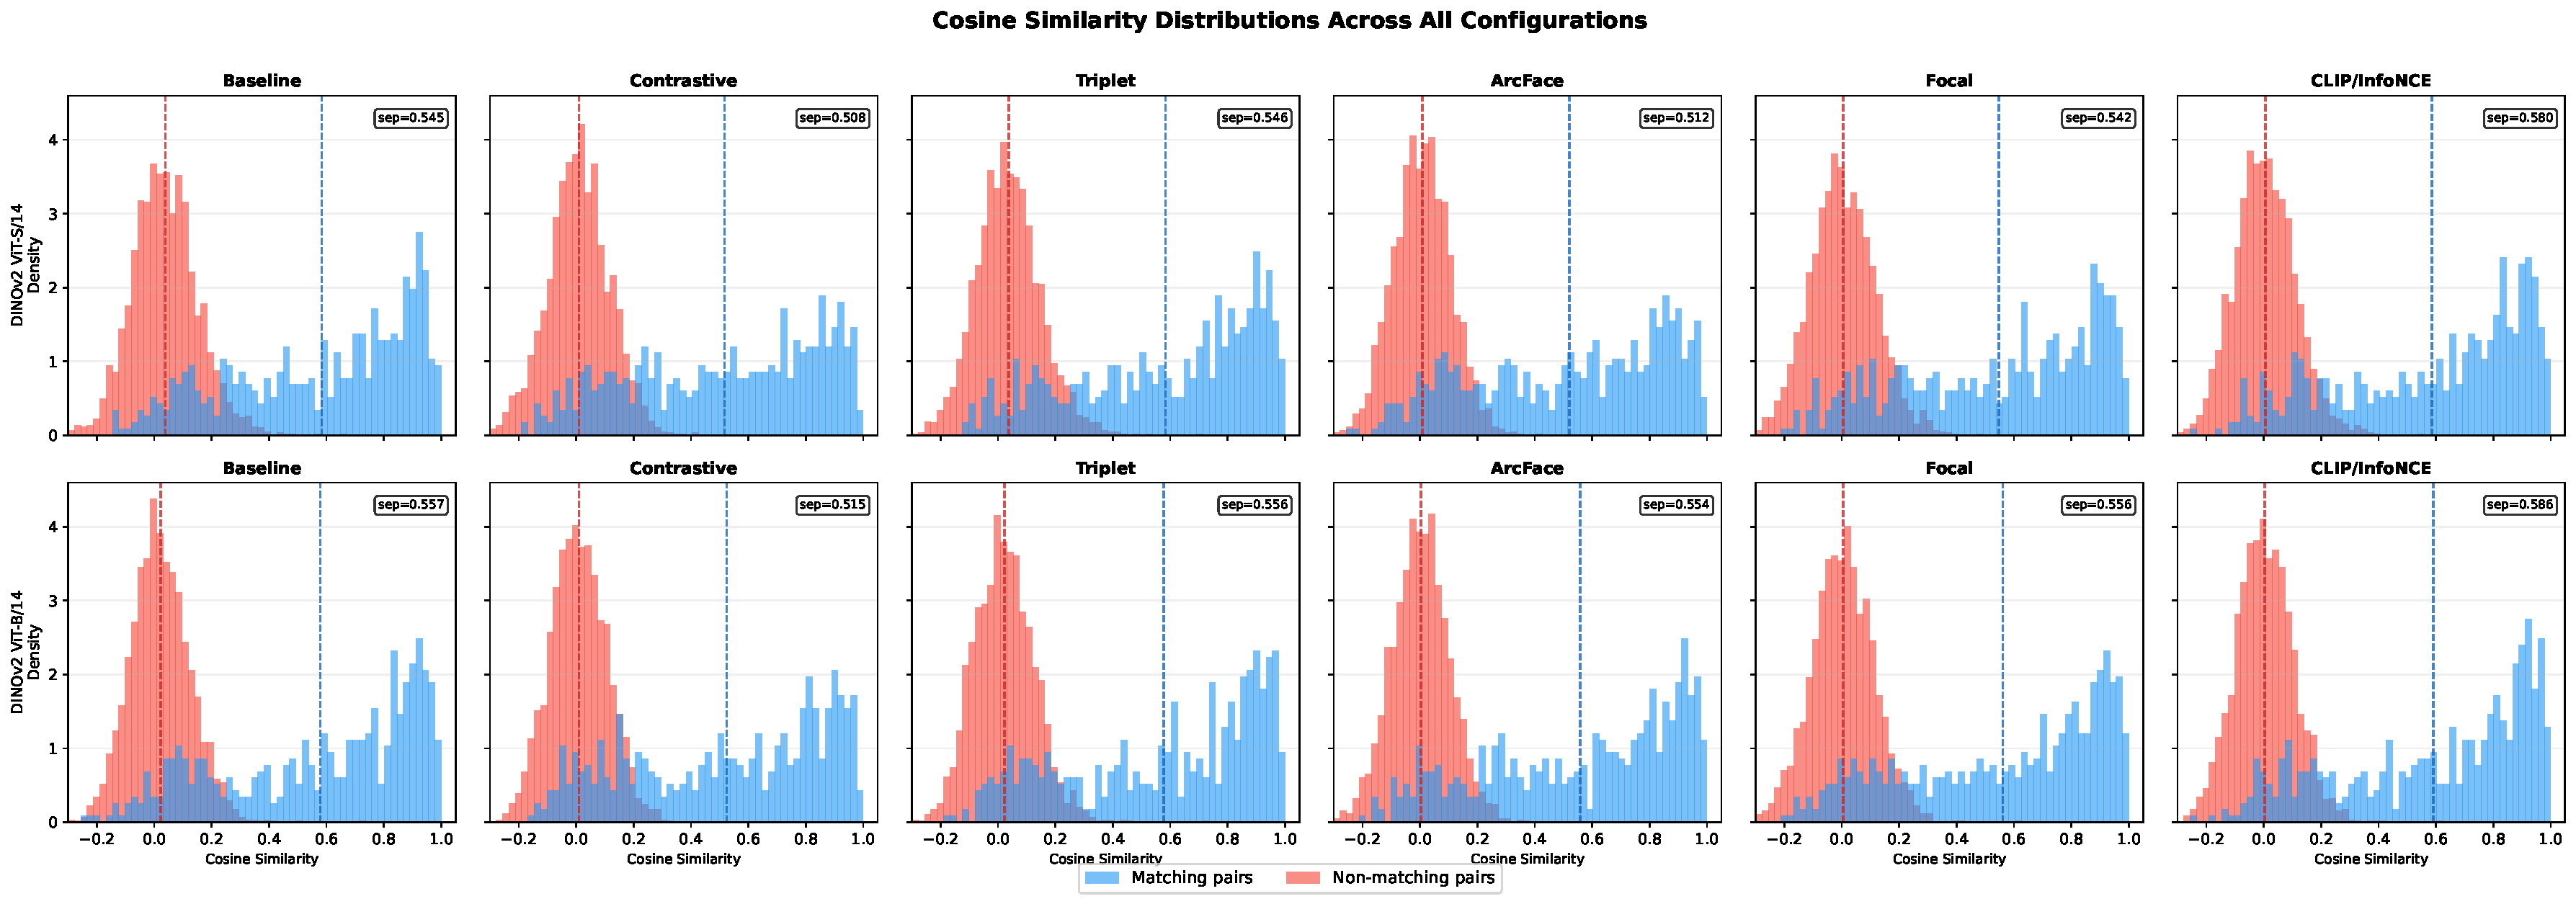
\includegraphics[width=\textwidth]{img/thesis_distance_grid.pdf}
    \caption{Cosine similarity distributions for all 12 configurations. Each panel shows matching pairs (correct query-reference pairs, blue) and non-matching pairs (random negatives, orange). Separation $\text{sep} = \bar{s}_{\text{match}} - \bar{s}_{\text{non-match}}$ is shown in each panel.}
    \label{fig:distance_grid}
\end{figure}

The distributions reveal a clear pattern: fine-tuning with classification-based losses (ArcFace, Focal, CLIP/InfoNCE) strongly compresses the non-matching distribution toward 0, reducing its mean from $\sim$0.038 (ViT-S baseline) to $\sim$0.004--0.006. This means the model learns to push unrelated images very close to the origin on the unit sphere, creating a large gap from matching pairs. The cosine similarity separation values confirm the ranking: ViT-B CLIP achieves the highest separation (0.586), followed by ViT-S CLIP (0.580), while contrastive-trained models on ViT-S show the most overlap between distributions (separation 0.508).

Figure~\ref{fig:umap_comparison} provides a qualitative view of three representative embedding spaces.

\begin{figure}[H]
    \centering
    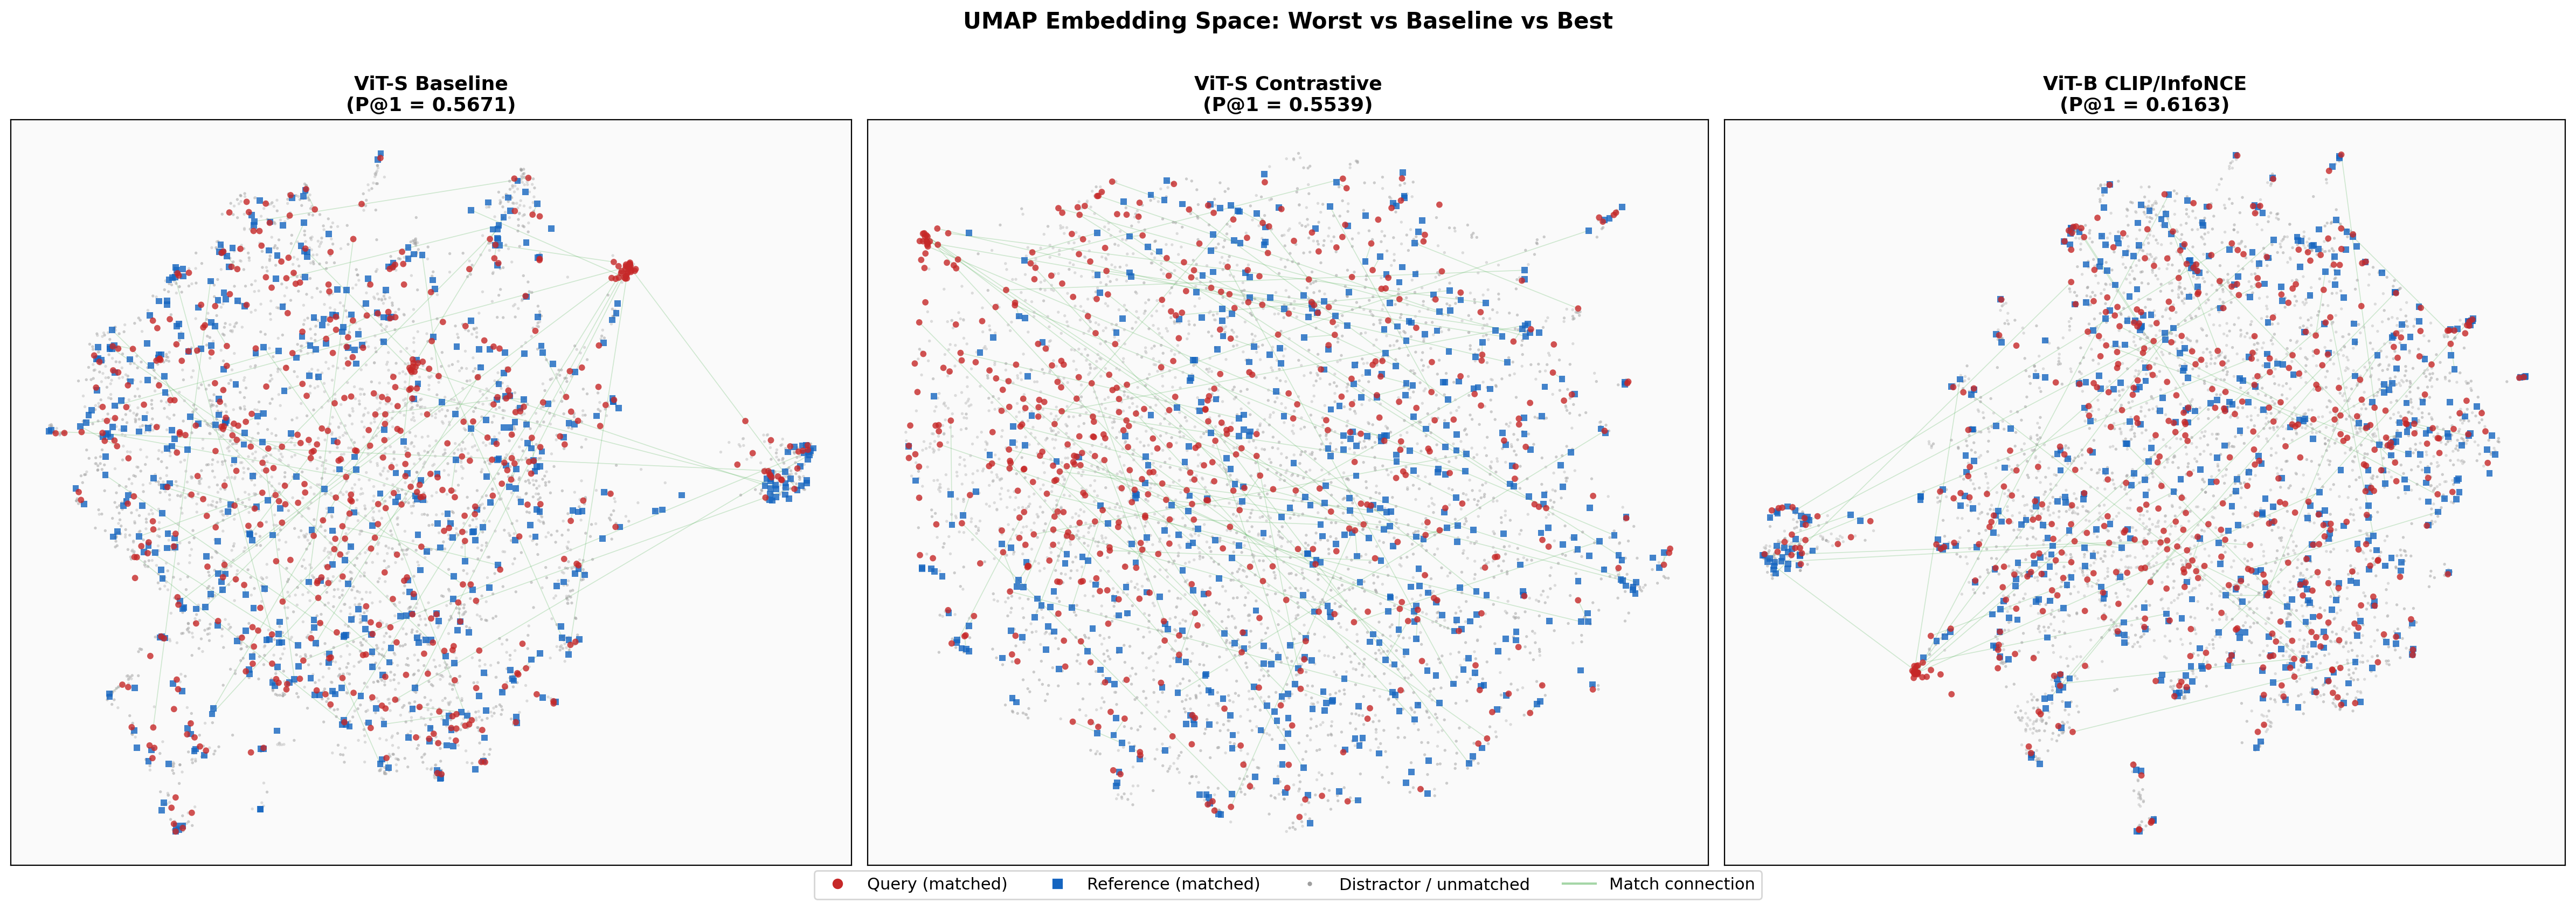
\includegraphics[width=\textwidth]{img/thesis_umap_comparison.png}
    \caption{UMAP projections of 500 development query embeddings for three representative configurations. Points are colored by whether the query's correct reference was retrieved at rank 1 (green: correct, red: incorrect). Left: ViT-S Baseline. Center: ViT-S Contrastive. Right: ViT-B CLIP/InfoNCE.}
    \label{fig:umap_comparison}
\end{figure}

The UMAP projections provide qualitative confirmation of the quantitative results. The ViT-B CLIP embedding space shows a more structured arrangement, with correct retrievals concentrated in denser regions, compared to the more scattered ViT-S baseline. It is important to note that UMAP projections are 2D approximations of high-dimensional spaces and should not be over-interpreted; the cosine similarity distributions and retrieval metrics remain the primary evidence.

\subsection{Discussion}

The experimental results reveal several important findings:

\textbf{1. Batch-level contrastive learning (CLIP/InfoNCE) is the most effective strategy.} The efficient use of all in-batch negatives provides a consistently superior learning signal compared to pairwise or triplet formulations, regardless of backbone size. The temperature parameter $\tau = 0.07$ plays a critical role in creating a sharp, discriminative distribution.

\textbf{2. Pre-training quality constrains triplet loss.} The failure of triplet loss on both backbones confirms that DINOv2's self-supervised pre-training already produces embeddings that satisfy standard margin constraints. Loss functions that do not depend on margin satisfaction (ArcFace, Focal, CLIP) are more suitable for fine-tuning highly capable pre-trained encoders.

\textbf{3. Backbone capacity changes the relative effectiveness of contrastive loss.} The reversal from ViT-S ($-$1.32 pp) to ViT-B (+2.46 pp) for contrastive loss suggests an interaction between backbone capacity and the loss formulation. Larger models may be better able to learn from the sparser supervision signal of pairwise contrastive training.

\textbf{4. Different metrics capture different retrieval behaviors.} Contrastive loss consistently improves $\mu$AP even when P@1 decreases, suggesting that it improves the ranking of correct matches in aggregate but not specifically at rank 1. Applications requiring strict top-1 accuracy should prefer CLIP/InfoNCE or ArcFace.

\textbf{5. Cosine similarity compression is a key geometric effect.} Classification-based losses (ArcFace, Focal, CLIP) strongly reduce the mean cosine similarity of non-matching pairs, creating a large separation between the two distributions. This geometric change is directly correlated with improved retrieval performance.

% ============================================================================
% REZULTATAI IR IŠVADOS (Results and Conclusions)
% ============================================================================
\sectionnonum{Results and Conclusions}

This work compared five metric learning loss functions—contrastive, triplet, ArcFace, Focal, and CLIP/InfoNCE—for fine-tuning two DINOv2 backbone variants (ViT-S/14 and ViT-B/14) on the image similarity task using the DISC21 dataset. A total of 12 experimental configurations were evaluated.

\textbf{Main results:}
\begin{enumerate}
    \item \textbf{CLIP/InfoNCE loss is the most effective loss function} for both backbone variants, achieving the best results overall: ViT-S P@1 = 60.49\% (+3.78 pp over ViT-S baseline) and ViT-B P@1 = 61.63\% (+3.79 pp over ViT-B baseline). Its batch-level contrastive formulation provides a richer learning signal than pairwise or triplet approaches.

    \item \textbf{Triplet loss is ineffective for both DINOv2 backbones.} Pre-trained embeddings already satisfy the margin constraint for all training triplets, resulting in zero loss and no gradient updates. This effect persists even with doubled margin and is independent of backbone size.

    \item \textbf{Contrastive loss is backbone-dependent.} On ViT-S it decreases P@1 below baseline; on ViT-B it achieves the second-best P@1 result (+2.46 pp). The larger backbone appears to have sufficient capacity to benefit from pairwise contrastive training.

    \item \textbf{ArcFace and Focal losses provide moderate, consistent improvements.} ArcFace achieves +1.70 pp P@1 on ViT-S and +1.33 pp on ViT-B. Focal loss provides smaller gains, as its hard-example focusing mechanism does not provide as strong a learning signal on this task.

    \item \textbf{ViT-B generally outperforms ViT-S} across all loss functions except triplet loss, where both fail to learn. The largest backbone benefit is seen with CLIP/InfoNCE and contrastive losses.
\end{enumerate}

\textbf{Conclusions:}
\begin{enumerate}
    \item For practical image similarity systems using pre-trained ViT encoders, CLIP/InfoNCE loss is the recommended fine-tuning objective due to its consistent superiority across both backbone sizes and evaluation metrics.

    \item Triplet loss is not suitable for fine-tuning highly capable pre-trained models like DINOv2. The pre-trained embedding space already satisfies standard margin constraints, making the loss function ineffective regardless of backbone size.

    \item Backbone capacity interacts with loss function choice. Contrastive loss benefits substantially from the larger ViT-B backbone while providing no benefit on ViT-S, indicating that the optimal loss function may depend on the model's representational capacity.

    \item Classification-based losses (ArcFace, Focal, CLIP/InfoNCE) produce a characteristic geometric effect: they strongly compress the non-matching similarity distribution toward 0, increasing the separation between matching and non-matching pairs. This effect is directly correlated with improved retrieval performance.
\end{enumerate}

\textbf{Limitations and future work:}
\begin{itemize}
    \item This study used a 50,000-image subset of DISC21 for training; experiments at full scale may yield different insights.
    \item The backbone was kept frozen throughout training. Unfreezing with careful learning rate scheduling (e.g., layer-wise learning rate decay) could potentially improve results, particularly for CLIP/InfoNCE.
    \item Only ViT-S and ViT-B were evaluated; larger variants (ViT-L at 307M, ViT-H at 632M) may show further gains.
    \item Combining loss functions (e.g., ArcFace + InfoNCE) or applying curriculum learning strategies could be explored.
    \item Final evaluation on the held-out DISC21 test set remains to be performed to report unbiased test performance.
\end{itemize}

% ============================================================================
% ŠALTINIAI (References)
% ============================================================================
\printbibliography[heading=bibintoc]

% ============================================================================
% PRIEDAI (Appendices)
% ============================================================================
\appendix{Detailed Training Logs}

This appendix provides the epoch-by-epoch training loss for all configurations, taken directly from the HPC training logs. The two backbone variants are shown separately.

\textbf{ViT-S/14 — Contrastive Loss:}
\begin{table}[H]
\centering
\small
\begin{tabular}{ccccc}
\toprule
\textbf{Epoch} & \textbf{Avg Loss} & \textbf{Epoch} & \textbf{Avg Loss} \\
\midrule
0 & 0.0788 & 10 & 0.0569 \\
1 & 0.0744 & 11 & 0.0568 \\
2 & 0.0765 & 12 & 0.0568 \\
3 & 0.0718 & 13 & 0.0601 \\
4 & 0.0709 & 14 & 0.0610 \\
5 & 0.0651 & 15 & 0.0569 \\
6 & 0.0654 & 16 & 0.0529 \\
7 & 0.0650 & 17 & 0.0606 \\
8 & 0.0621 & 18 & 0.0529 \\
9 & 0.0603 & 19 & 0.0537 \\
\bottomrule
\end{tabular}
\caption{ViT-S Contrastive loss training progression}
\end{table}

\textbf{ViT-S/14 — Triplet Loss:}
\begin{table}[H]
\centering
\small
\begin{tabular}{ccccc}
\toprule
\textbf{Epoch} & \textbf{Avg Loss} & \textbf{Epoch} & \textbf{Avg Loss} \\
\midrule
0 & 0.0 & 10 & 0.0 \\
1 & 0.0 & 11 & 0.0 \\
2 & 0.0 & 12 & 0.0 \\
3 & 0.0 & 13 & 0.0 \\
4 & 0.0 & 14 & 0.0 \\
5 & 0.0 & 15 & 0.0 \\
6 & 0.0 & 16 & 0.0 \\
7 & 0.0 & 17 & 0.0 \\
8 & 0.0 & 18 & 0.0 \\
9 & 0.0 & 19 & 0.0 \\
\bottomrule
\end{tabular}
\caption{ViT-S Triplet loss training progression ($m = 0.5$). Loss remained 0.0 throughout because the hard triplet miner found no margin-violating triplets. A follow-up with $m = 1.0$ produced identical results. ViT-B Triplet (not shown) also remained 0.0 for all epochs.}
\end{table}

\textbf{ViT-S/14 — ArcFace Loss:}
\begin{table}[H]
\centering
\small
\begin{tabular}{ccccc}
\toprule
\textbf{Epoch} & \textbf{Avg Loss} & \textbf{Epoch} & \textbf{Avg Loss} \\
\midrule
0 & 27.36 & 10 & 0.90 \\
1 & 21.53 & 11 & 0.72 \\
2 & 16.88 & 12 & 0.59 \\
3 & 12.90 & 13 & 0.51 \\
4 & 9.33  & 14 & 0.45 \\
5 & 6.33  & 15 & 0.41 \\
6 & 4.06  & 16 & 0.39 \\
7 & 2.58  & 17 & 0.37 \\
8 & 1.71  & 18 & 0.36 \\
9 & 1.20  & 19 & 0.35 \\
\bottomrule
\end{tabular}
\caption{ViT-S ArcFace loss training progression}
\end{table}

\textbf{ViT-S/14 — Focal Loss:}
\begin{table}[H]
\centering
\small
\begin{tabular}{ccccc}
\toprule
\textbf{Epoch} & \textbf{Avg Loss} & \textbf{Epoch} & \textbf{Avg Loss} \\
\midrule
0 & 13.0654 & 10 & 0.0038 \\
1 & 6.7261  & 11 & 0.0029 \\
2 & 2.1969  & 12 & 0.0029 \\
3 & 0.3186  & 13 & 0.0027 \\
4 & 0.0625  & 14 & 0.0023 \\
5 & 0.0219  & 15 & 0.0023 \\
6 & 0.0108  & 16 & 0.0021 \\
7 & 0.0067  & 17 & 0.0020 \\
8 & 0.0050  & 18 & 0.0020 \\
9 & 0.0044  & 19 & 0.0020 \\
\bottomrule
\end{tabular}
\caption{ViT-S Focal loss training progression. Rapid convergence in the first few epochs is characteristic of focal loss with $\gamma = 2$.}
\end{table}

\textbf{ViT-S/14 — CLIP/InfoNCE Loss:}
\begin{table}[H]
\centering
\small
\begin{tabular}{ccccc}
\toprule
\textbf{Epoch} & \textbf{Avg Loss} & \textbf{Epoch} & \textbf{Avg Loss} \\
\midrule
0 & 0.0626 & 10 & 0.0243 \\
1 & 0.0426 & 11 & 0.0241 \\
2 & 0.0376 & 12 & 0.0236 \\
3 & 0.0343 & 13 & 0.0237 \\
4 & 0.0312 & 14 & 0.0234 \\
5 & 0.0298 & 15 & 0.0226 \\
6 & 0.0279 & 16 & 0.0226 \\
7 & 0.0271 & 17 & 0.0233 \\
8 & 0.0260 & 18 & 0.0226 \\
9 & 0.0260 & 19 & 0.0216 \\
\bottomrule
\end{tabular}
\caption{ViT-S CLIP/InfoNCE loss training progression. The implementation uses a normalized pairwise formulation; the resulting scale differs from the raw InfoNCE formulation described in Section~\ref{sec:similarity_search}.}
\end{table}

\textbf{ViT-B/14 — Contrastive Loss:}
\begin{table}[H]
\centering
\small
\begin{tabular}{ccccc}
\toprule
\textbf{Epoch} & \textbf{Avg Loss} & \textbf{Epoch} & \textbf{Avg Loss} \\
\midrule
0 & 0.0941 & 10 & 0.0708 \\
1 & 0.0938 & 11 & 0.0670 \\
2 & 0.0970 & 12 & 0.0713 \\
3 & 0.0866 & 13 & 0.0591 \\
4 & 0.0777 & 14 & 0.0592 \\
5 & 0.0732 & 15 & 0.0592 \\
6 & 0.0793 & 16 & 0.0599 \\
7 & 0.0793 & 17 & 0.0578 \\
8 & 0.0726 & 18 & 0.0610 \\
9 & 0.0717 & 19 & 0.0633 \\
\bottomrule
\end{tabular}
\caption{ViT-B Contrastive loss training progression}
\end{table}

\textbf{ViT-B/14 — ArcFace Loss:}
\begin{table}[H]
\centering
\small
\begin{tabular}{ccccc}
\toprule
\textbf{Epoch} & \textbf{Avg Loss} & \textbf{Epoch} & \textbf{Avg Loss} \\
\midrule
0 & 27.72 & 10 & 1.48 \\
1 & 23.07 & 11 & 1.14 \\
2 & 18.78 & 12 & 0.93 \\
3 & 15.00 & 13 & 0.79 \\
4 & 11.61 & 14 & 0.69 \\
5 & 8.62  & 15 & 0.62 \\
6 & 6.10  & 16 & 0.57 \\
7 & 4.15  & 17 & 0.54 \\
8 & 2.83  & 18 & 0.53 \\
9 & 1.99  & 19 & 0.52 \\
\bottomrule
\end{tabular}
\caption{ViT-B ArcFace loss training progression}
\end{table}

\textbf{ViT-B/14 — Focal Loss:}
\begin{table}[H]
\centering
\small
\begin{tabular}{ccccc}
\toprule
\textbf{Epoch} & \textbf{Avg Loss} & \textbf{Epoch} & \textbf{Avg Loss} \\
\midrule
0 & 13.4157 & 10 & 0.0057 \\
1 & 8.3542  & 11 & 0.0049 \\
2 & 3.9764  & 12 & 0.0043 \\
3 & 0.9451  & 13 & 0.0038 \\
4 & 0.1566  & 14 & 0.0040 \\
5 & 0.0474  & 15 & 0.0037 \\
6 & 0.0225  & 16 & 0.0032 \\
7 & 0.0133  & 17 & 0.0032 \\
8 & 0.0091  & 18 & 0.0030 \\
9 & 0.0073  & 19 & 0.0031 \\
\bottomrule
\end{tabular}
\caption{ViT-B Focal loss training progression}
\end{table}

\textbf{ViT-B/14 — CLIP/InfoNCE Loss:}
\begin{table}[H]
\centering
\small
\begin{tabular}{ccccc}
\toprule
\textbf{Epoch} & \textbf{Avg Loss} & \textbf{Epoch} & \textbf{Avg Loss} \\
\midrule
0 & 0.0391 & 10 & 0.0169 \\
1 & 0.0299 & 11 & 0.0171 \\
2 & 0.0259 & 12 & 0.0163 \\
3 & 0.0240 & 13 & 0.0161 \\
4 & 0.0225 & 14 & 0.0158 \\
5 & 0.0197 & 15 & 0.0156 \\
6 & 0.0196 & 16 & 0.0159 \\
7 & 0.0186 & 17 & 0.0153 \\
8 & 0.0178 & 18 & 0.0152 \\
9 & 0.0175 & 19 & 0.0150 \\
\bottomrule
\end{tabular}
\caption{ViT-B CLIP/InfoNCE loss training progression}
\end{table}

\appendix{Experimental Environment}

All experiments were conducted using the following hardware and software configuration:

\textbf{Hardware:}
\begin{itemize}
    \item \textbf{HPC Cluster}: VU MIF HPC (Vilnius University)
    \item \textbf{GPU}: NVIDIA Tesla V100 (32GB HBM2)
    \item \textbf{CPU}: Intel Xeon (4 cores allocated per job)
    \item \textbf{RAM}: 64GB per job
\end{itemize}

\textbf{Software:}
\begin{itemize}
    \item \textbf{Python}: 3.10
    \item \textbf{PyTorch}: 2.0 with CUDA 11.8
    \item \textbf{PyTorch Metric Learning}: 2.3.0
    \item \textbf{DINOv2}: torch.hub (\texttt{dinov2\_vits14}, \texttt{dinov2\_vitb14})
    \item \textbf{umap-learn}: 0.5.3 (embedding visualization)
\end{itemize}

\textbf{Training Time (approximate, on V100 32GB):}
\begin{itemize}
    \item Baseline evaluation (ViT-S or ViT-B): $\sim$10 minutes
    \item Contrastive / CLIP training, ViT-S (20 epochs): $\sim$2.5 hours
    \item ArcFace / Focal / Triplet training, ViT-S (20 epochs): $\sim$1.7 hours
    \item Contrastive / CLIP training, ViT-B (20 epochs): $\sim$2.8 hours
    \item ArcFace / Focal / Triplet training, ViT-B (20 epochs): $\sim$1.8 hours
\end{itemize}

\end{document}
